% Template for PLoS
% Version 3.6 Aug 2022
%
% % % % % % % % % % % % % % % % % % % % % %
%
% -- IMPORTANT NOTE
%
% This template contains comments intended 
% to minimize problems and delays during our production 
% process. Please follow the template instructions
% whenever possible.
%
% % % % % % % % % % % % % % % % % % % % % % % 
%
% Once your paper is accepted for publication, 
% PLEASE REMOVE ALL TRACKED CHANGES in this file 
% and leave only the final text of your manuscript. 
% PLOS recommends the use of latexdiff to track changes during review, as this will help to maintain a clean tex file.
% Visit https://www.ctan.org/pkg/latexdiff?lang=en for info or contact us at latex@plos.org.
%
%
% There are no restrictions on package use within the LaTeX files except that no packages listed in the template may be deleted.
%
% Please do not include colors or graphics in the text.
%
% The manuscript LaTeX source should be contained within a single file (do not use \input, \externaldocument, or similar commands).
%
% % % % % % % % % % % % % % % % % % % % % % %
%
% -- FIGURES AND TABLES
%
% Please include tables/figure captions directly after the paragraph where they are first cited in the text.
%
% DO NOT INCLUDE GRAPHICS IN YOUR MANUSCRIPT
% - Figures should be uploaded separately from your manuscript file. 
% - Figures generated using LaTeX should be extracted and removed from the PDF before submission. 
% - Figures containing multiple panels/subfigures must be combined into one image file before submission.
% For figure citations, please use "Fig" instead of "Figure".
% See http://journals.plos.org/plosone/s/figures for PLOS figure guidelines.
%
% Tables should be cell-based and may not contain:
% - spacing/line breaks within cells to alter layout or alignment
% - do not nest tabular environments (no tabular environments within tabular environments)
% - no graphics or colored text (cell background color/shading OK)
% See http://journals.plos.org/plosone/s/tables for table guidelines.
%
% For tables that exceed the width of the text column, use the adjustwidth environment as illustrated in the example table in text below.
%
% % % % % % % % % % % % % % % % % % % % % % % %
%
% -- EQUATIONS, MATH SYMBOLS, SUBSCRIPTS, AND SUPERSCRIPTS
%
% IMPORTANT
% Below are a few tips to help format your equations and other special characters according to our specifications. For more tips to help reduce the possibility of formatting errors during conversion, please see our LaTeX guidelines at http://journals.plos.org/plosone/s/latex
%
% For inline equations, please be sure to include all portions of an equation in the math environment.  For example, x$^2$ is incorrect; this should be formatted as $x^2$ (or $\mathrm{x}^2$ if the romanized font is desired).
%
% Do not include text that is not math in the math environment. For example, CO2 should be written as CO\textsubscript{2} instead of CO$_2$.
%
% Please add line breaks to long display equations when possible in order to fit size of the column. 
%
% For inline equations, please do not include punctuation (commas, etc) within the math environment unless this is part of the equation.
%
% When adding superscript or subscripts outside of brackets/braces, please group using {}.  For example, change "[U(D,E,\gamma)]^2" to "{[U(D,E,\gamma)]}^2". 
%
% Do not use \cal for caligraphic font.  Instead, use \mathcal{}
%
% % % % % % % % % % % % % % % % % % % % % % % % 
%
% Please contact latex@plos.org with any questions.
%
% % % % % % % % % % % % % % % % % % % % % % % %

\documentclass[10pt,letterpaper]{article}
\usepackage[top=0.85in,left=2.75in,footskip=0.75in]{geometry}

% amsmath and amssymb packages, useful for mathematical formulas and symbols
\usepackage{amsmath,amssymb}

% Use adjustwidth environment to exceed column width (see example table in text)
\usepackage{changepage}

% textcomp package and marvosym package for additional characters
\usepackage{textcomp,marvosym}

% cite package, to clean up citations in the main text. Do not remove.
\usepackage{cite}

% Use nameref to cite supporting information files (see Supporting Information section for more info)
\usepackage{nameref,hyperref}

% line numbers
\usepackage[right]{lineno}

% ligatures disabled
% \usepackage[nopatch=eqnum]{microtype}
% \DisableLigatures[f]{encoding = *, family = * }

% color can be used to apply background shading to table cells only
\usepackage[table]{xcolor}

% array package and thick rules for tables
\usepackage{array}

% graphicx package
\usepackage{graphicx}

%Path relative to the main .tex file 
\graphicspath{ {./figures/} }

% create "+" rule type for thick vertical lines
\newcolumntype{+}{!{\vrule width 2pt}}

% create \thickcline for thick horizontal lines of variable length
\newlength\savedwidth
\newcommand\thickcline[1]{%
  \noalign{\global\savedwidth\arrayrulewidth\global\arrayrulewidth 2pt}%
  \cline{#1}%
  \noalign{\vskip\arrayrulewidth}%
  \noalign{\global\arrayrulewidth\savedwidth}%
}

% \thickhline command for thick horizontal lines that span the table
\newcommand\thickhline{\noalign{\global\savedwidth\arrayrulewidth\global\arrayrulewidth 2pt}
\hline
\noalign{\global\arrayrulewidth\savedwidth}}


% Remove comment for double spacing
%\usepackage{setspace} 
%\doublespacing

% Text layout
\raggedright
\setlength{\parindent}{0.5cm}
\textwidth 5.25in 
\textheight 8.75in

% Bold the 'Figure #' in the caption and separate it from the title/caption with a period
% Captions will be left justified
\usepackage[aboveskip=1pt,labelfont=bf,labelsep=period,justification=raggedright,singlelinecheck=off]{caption}
\renewcommand{\figurename}{Fig}

% Use the PLoS provided BiBTeX style
\bibliographystyle{plos2015}


% Remove brackets from numbering in List of References
\makeatletter
\renewcommand{\@biblabel}[1]{\quad#1.}
\makeatother



% Header and Footer with logo
\usepackage{lastpage,fancyhdr,graphicx}
\usepackage{epstopdf}
%\pagestyle{myheadings}
\pagestyle{fancy}
\fancyhf{}
%\setlength{\headheight}{27.023pt}
%\lhead{\includegraphics[width=2.0in]{PLOS-submission.eps}}
\rfoot{\thepage/\pageref{LastPage}}
\renewcommand{\headrulewidth}{0pt}
\renewcommand{\footrule}{\hrule height 2pt \vspace{2mm}}
\fancyheadoffset[L]{2.25in}
\fancyfootoffset[L]{2.25in}
\lfoot{\today}

%% Include all macros below

\newcommand{\lorem}{{\bf LOREM}}
\newcommand{\ipsum}{{\bf IPSUM}}

%% END MACROS SECTION


\begin{document}
\vspace*{0.2in}

% Title must be 250 characters or less.
\begin{flushleft}
{\Large
\textbf\newline{Time-series modeling of epidemics in complex populations: detecting changes in incidence dispersion over time} % Please use "sentence case" for title and headings (capitalize only the first word in a title (or heading), the first word in a subtitle (or subheading), and any proper nouns).
}
\newline
% Insert author names, affiliations and corresponding author email (do not include titles, positions, or degrees).
\\
Rachael Aber\textsuperscript{1,2},
Yanming Di\textsuperscript{2},
Benjamin Dalziel\textsuperscript{1, 3},
\\
\bigskip
\textbf{1} Department of Integrative Biology, Oregon State University, Corvallis, Oregon, USA
\\
\textbf{2} Department of Statistics, Oregon, Oregon State University, Corvallis, Oregon, USA
\\
\textbf{3} Department of Mathematics, Oregon State University, Corvallis, Oregon, USA
\bigskip

% Insert additional author notes using the symbols described below. Insert symbol callouts after author names as necessary.
% 
% Remove or comment out the author notes below if they aren't used.
%
% Primary Equal Contribution Note
% \Yinyang These authors contributed equally to this work.

% Additional Equal Contribution Note
% Also use this double-dagger symbol for special authorship notes, such as senior authorship.
% \ddag These authors also contributed equally to this work.

% Current address notes
%%\textcurrency Current Address: Dept/Program/Center, Institution Name, City, State, Country % change symbol to "\textcurrency a" if more than one current address note
% \textcurrency b Insert second current address 
% \textcurrency c Insert third current address

% Deceased author note
% \dag Deceased

% Group/Consortium Author Note
%\textpilcrow Membership list can be found in the Acknowledgments section.

% Use the asterisk to denote corresponding authorship and provide email address in note below.
* aberr@oregonstate.edu

\end{flushleft}
% Please keep the abstract below 300 words
\section*{Abstract}
Trends in infectious disease incidence provide important information about epidemic dynamics and prospects for control. 
Higher-frequency variation around incidence trends can shed light on the processes driving transmission in complex populations, as transmission heterogeneity, shifting landscapes of susceptibility, and fluctuations in reporting can directly impact the volatility of observed case counts.
However, measures of incidence variability--and how they change over time--are often overlooked in population-level analyses of incidence data.
Here we present a statistical framework to quantify temporal changes in incidence dispersion and detect discrete shifts in the dispersion parameter, which may signal new epidemic phases. 
We apply the method to COVID-19 case count data in 144 US counties from the January 1st, 2020 to March 23rd, 2023.
While standard theory predicts that dispersion should be inversely proportional to incidence, our method reveals pronounced temporal trends in dispersion that are not explained by incidence alone, but which are replicated across counties. 
Dispersion increased around the major surge in cases in 2022, and highly overdispersed patterns became more frequent later in the time series.
These findings suggest that heterogeneity in transmission, susceptibility, and reporting may play causal roles in driving large surges and extending epidemic duration. 
The dispersion of incidence time series can contain structured information which enhances predictive understanding of the underlying drivers of transmission, with applications as leading indicators for public health response.



% Please keep the Author Summary between 150 and 200 words
% Use first person. PLOS ONE authors please skip this step. 
% Author Summary not valid for PLOS ONE submissions.   
\section*{Author summary}
Understanding patterns in infectious disease incidence is crucial for understanding epidemic dynamics and for developing effective public health responses. 
However, traditional metrics used to quantify incidence patterns often overlook variability as an important characteristic of incidence time series. 
Quantifying higher-frequency variation around incidence trends can elucidate important underlying processes, including transmission heterogeneity or changes in the susceptibility landscape.
We developed a statistical framework to quantify temporal changes in case count dispersion within a single time series. 
We used negative binomial regression to account for factors that might confound the estimation of dispersion, allowing us to use a single parameter to infer the degree of case count dispersion. 
We applied the method to COVID-19 case count data from 144 US counties from January 1st, 2020 to March 23rd, 2023, and found that conspicuous shifts in dispersion occurred across counties concurrently, and that these shifts were not explained by incidence alone. 
Dispersion increased around peaks in incidence such as the major surge in cases in 2022, and dispersion also increased as the pandemic progressed. 
These increases potentially indicate that some individuals spread SARS-CoV-2 (the virus that causes COVID-19) to many more people than others, that the susceptibility landscape changed, or that there were changes in reporting.
Shifts in dispersion can indicate shifts in epidemic phase as well as provide information about important underlying biological processes. 
Therefore, our method to estimate dispersion provides a way for public health officials to anticipate and manage changes in epidemic regime and the drivers of transmission. 

\linenumbers

% Use "Eq" instead of "Equation" for equation citations.
\section*{Introduction}
Time series of infectious disease incidence appear, to varying degrees, ``noisy'', showing higher frequency fluctuations (e.g., day-to-day or week-to-week fluctations) around trends at the broader temporal ranges typical for epidemic curves (e.g., months or years).
Short-term fluctuations in incidence time series are often caused in part by variable reporting, but also reflect the population-level impacts of transmission heterogeneity, and/or changes in susceptiblility~\cite{lloyd-smith_superspreading_2005, kirkegaard_superspreading_2021, sun_transmission_2021,guo2023statistical,ko2023time}.
Metrics of variability in incidence time series could therefore carry information regarding underlying drivers of transmission, and offer a relatively unexplored avenue for understanding epidemic dynamics. 

``Metrics of variability'' are estimates of the extent to which incidence is dispersed relative to its expected value.
The expectation could be provided by a moving average of past incidence, a process-based model, or another type of population-level model. 
While the expectation itself will vary over time, there may also be important variation in the level of dispersion around the deterministic skeleton of the epidemic. 
Individual-level heterogeneity in transmission scales up to affect population-level dynamics \cite{lloyd-smith_superspreading_2005}, so variability in epidemic trajectories at the population level may provide information about individual-level variability in the transmission process (transmission heterogeneity).

Contact tracing data has revealed temporal variation in transmission heterogeneity, which is quantified using the dispersion parameter of the offspring distribution.
Working from contact tracing data, researchers found that the dispersion parameter of the offspring distribution varied during different phases of the COVID-19 epidemic in Hong Kong \cite{guo2023statistical}, which is important for understanding and managing the population-level dynamics of disease transmission and outbreak control.
Similarly, the dispersion parameter of the offspring distribution varied over time as new variants emerged \cite{ko2023time}. 
However, traditional contact tracing is very resource intensive, and although new approaches using digital technologies may improve its speed and availability \cite{kretzschmar_impact_2020}, there is a need for complementary population-level analyses that can estimate heterogeneity using incidence data, which is more widely available. The importance of considering population-level variability and its relationship to individual-level variability is further highlighted by the finding that a combination of individual-based and population-based strategies was required for SARS-CoV-2 control \cite{sun_transmission_2021}. 

Statistical techniques that make inference based on the variability of epidemic time series at the population level are emerging. Working from population-level incidence data, the offspring distribution dispersion parameter was estimated \cite{kirkegaard_superspreading_2021}.
Another area of interest is how incidence variability is related to different phases of an epidemic. For example, the mean and interannual coefficient of variation of measles incidence was used to construct a metric indicative of where a location may be on the path to elimination of a pathogen~\cite{graham_measles_2019}. 
Analyzing variability in terms of bursts of incidence is also important for planning surge capacity in public health systems\cite{wallinga_metropolitan_2018}. 
Dispersion is a way to specifically capture clustering of cases in epidemic time series. An index of effective aggregate dispersion (EffDI) was proposed to elucidate clusters of infection directly from incidence data \cite{schneckenreither_assessing_2023}. In the current work, our interest is in the dispersion of epidemic time series.

Incidence dispersion dynamics are distinct from, but related to, the dispersion parameter of the offspring distribution. 
Infectious disease transmission follows a branching process, as new infections result from exposure to individuals who are currently infectious. 
Under a wide range of configurations for a branching process model, including the vast majority of parsimonious ones, the number of infected individuals $I_t$ at time $t$ will have a negative binomial distribution \cite{kendall_stochastic_1949}: $I_t \sim NB \left( \mu_t, \theta_t \right)$, where $\mu_t$ is the expected value for $I_t$ and $\theta_t$ is the dispersion parameter. 
The dispersion parameter is related to the variance of incidence by $\mathrm{Var}[I_t] = \mu_t + \mu_t^2 / \theta_t$. 
Importantly, smaller values of the dispersion parameter $\theta_t$ correspond to increasing amounts of dispersion, increasing amounts by which the variance in realized number infected $I_t$ exceeds the expected value, $\mu_t$. 
Conversely, the distribution of $I_t$ tends to a Poisson distribution (where the variance equals mean) as $\theta_t$ becomes large. 
This model is common in population biology (e.g., in the study of measles \cite{grenfell_dynamics_2002}).

An interpretation of the dispersion parameter for a time series model of counts is that events are $1 + \theta^{-1}$ times as ``crowded" in time relative to a Poisson process with the same mean \cite{lloyd_mean_1967}. For example, $\theta = 1$ corresponds to a situation where the average number of infections in the same time step as a randomly selected case will exceed the Poisson expectation by a factor of two. In a simple example relevant to surge capacity in the healthcare system, $\theta = 1$ implies that a random infectious individual visiting the emergency department at a hospital would find it on average to be twice as crowded with other infectious individuals (infected by the same pathogen) than expected for a Poisson process with the same incidence rate.

Modeling $\mu_t$ and $\theta_t$ is important to the prediction of epidemics. A time-series approximation to compartment epidemic models uses $\mu_t = \lambda I_{t-1}$ where $\lambda$ is the current local rate at which incidence at time $t-1$ produces new infections at time $t$ and $\theta_t = I_{t-1}$. 
\begin{equation}
    \mathrm{I_t} = NB(\mu = \lambda I_{t-1}, \theta_t = I_{t-1})
\end{equation}
The assertion that $\theta_t = I_{t-1}$ comes from the assumption that each of the individuals who acquired the infection at $t-1$ form ``independent lineages'' with identically distributed ``local'' rate parameter. Under these conditions, $\theta_t = I_{t-1}$ is a good approximation for sufficiently large populations (\cite{kendall_stochastic_1949}, \cite{bjornstad_dynamics_nodate}). However, this model assumes that subpopulations of infectious individuals emanating from one infected individuals are independent and statistically identical to those from another. That is, the model assumes susceptible depletion in one lineage does not affect another, transmission rates are equal across lineages, and reporting rates do not vary across lineages. 

In practice, the above assumptions may not hold, so we instead estimate $\theta_t$ to understand how heterogeneity in transmission, susceptibility and reporting (and other factors) are driving epidemic dynamics. 
Instead of assuming $\theta_t = I_{t-1}$, drivers of $\theta_t$ can be investigated, first by quantifying how it changes over time and to what degree it is governed by $I_t$. 
We adopt a more general/phenomenological model for $\mu_t$. 
Instead of $\mu_t = \lambda I_{t-1}$, which is a special kind of moving window, we use a spline which is able to approximate the solution to a wider range of autoregressive and other models. 
Furthermore, the rate of the case-count-generating process is often changing within a time step, which cannot be accommodated by a Poisson model. 
The negative binomial distribution may accurately model a time series if there is a changing process mean within a time step: for example, if the mean of a Poisson distribution itself follows a gamma distribution, the resulting distribution is negative binomial \cite{cook_notes_nodate}. 
This is an additional reason that the dispersion parameter of a negative binomial distribution should be used to measure changes in meaningful case count clustering in settings with differing base population/incidence. 
Negative binomial regression (in contrast to Poisson regression) can account for unobserved heterogeneity, time dependence in the rate of a process and contagion within a time step that all lead to overdispersion \cite{barron_analysis_1992}.

We develop a method that quantifies the evolution of dispersion along incidence time series, allowing for the detection of changes in clustering that are not due to changes in population size or overall burden of incidence.
We apply the method to COVID-19 incidence data in US counties to investigate the relationships between incidence, dispersion and epidemic dynamic regimes over a portion of the COVID-19 pandemic. 

\section*{Materials and methods}
\subsection*{Introduction to the method}

% For figure citations, please use "Fig" instead of "Figure".
Classical approaches \cite{grenfell_dynamics_2002} model incidence at a time step using a negative binomial variable with expectation equal to the epidemic intensity and dispersion parameter equal to previous incidence. However, other processes besides the current number infected might affect dispersion, so we instead investigate changes in dispersion over time to understand processes that may leave a signal in dispersion. 

Our general framework is that incidence at a time step is drawn from a negative binomial distribution with time-varying mean and dispersion parameter (the dispersion parameter varies more slowly than the mean parameter). 
The model is formulated with a linear predictor that includes a natural spline in time with three degrees of freedom to account for autocorrelation in case counts. 
Natural splines are cubic splines which are linear outside of the boundary knots \cite{perperoglou_review_2019}. 
A recently proposed negative binomial regression model for time series of counts also accommodates serial dependence \cite{davis_negative_2009}. 

A persistent challenge in investigating changes in variability has been ``spurious correlation'' with population size. 
Since population size influences the mean and variance of case count data and thus could have an impact on estimates of dispersion, we adjust for population size using an offset in the model. 
There is an offset term in order to directly model counts (here, COVID-19 cases) per unit of observation (here, per individual).

\begin{align}
  \log(E[Y_i]/n_i) &= \beta_1h_1(t_i) + \beta_2h_2(t_i) + \beta_3h_3(t_i) \\
  \log(E[Y_i])-\log(n_i) &= \beta_1h_1(t_i) + \beta_2h_2(t_i) + \beta_3h_3(t_i) \\ 
  \log(E[Y_i]) &= \beta_1 h_1(t_i) + \beta_2h_2(t_i) + \beta_3 h_3(t_i) + log(n_i) 
\end{align}

Thus, the form of the probability mass function for incidence at a time step is:

\begin{equation}
  f_t(I) = \binom{I + \theta - 1}{I} \left(\dfrac{\mu}{\mu+\theta}\right)^I \left(\dfrac{\theta}{\mu +\theta}\right)^\theta
\end{equation}

where \begin{math}\mu\end{math} for the time step is estimated via the linear predictor outlined above.

The form of the expectation and variance from this model is below.

\begin{align}
  E(I) &= \mu\\
  Var(I) &= \mu + \dfrac{\mu^2}{\theta}
\end{align}

Note that high variability/dispersion corresponds to low values of the dispersion parameter, \begin{math}\theta\end{math}.
In sum, our method identifies shifts in population-level dispersion in incidence while accounting for population size. 
In addition to fitting the model at each time step, we developed a straightforward likelihood-ratio test (LRT) that could be applied at each time step. This involves fitting both a null model (no \begin{math}\theta\end{math} change) and a two-part (\begin{math}\theta\end{math}-change) model.

\subsection*{Application to simulated data}

To test the validity and power of the LRT, we simulated both Gaussian and uniform epidemic curves with an attack rate of 0.1--epidemic curves over 60 time steps each were produced, and the likelihood-ratio test (LRT) procedure was applied to each. 
Varying the magnitude of the \begin{math}\theta\end{math} change, location of the change in the curve, population size underlying the curve, and curve shape (as mentioned above) allowed us to test the validity and power of our approach across a range of situations.

\subsection*{Application to empirical data}
%To evaluate whether the negative binomial conditional distribution is needed (opposed to a Poisson/quasi-Poisson conditional distribution with the same model of process mean), inspection of mean-variance relationships using a diagnostic plot is possible \cite{ver_hoef_quasi-poisson_2007}, along with evaluation of dispersion statistics.
We estimated \begin{math}\mu_t\end{math} and one \begin{math}\theta\end{math} using iteratively reweighted least-squares (procedure implemented via the NBPSeq R package \cite{NBPSeq}) using a window around each time step.
For each window, \begin{math}\mu_t\end{math} was estimated using a spline function in time, and the single value of \begin{math}\theta\end{math} was estimated for that window. 
By moving the window one time step at a time, a time series of \begin{math}\theta_t\end{math} was produced. We investigated large counties (the largest three counties in each state), due to power constraints.

% Results and Discussion can be combined.
\section*{Results}
We found that the LRT method is robust across population sizes (for population sizes included in the empirical data) (Fig.\ 1 e, f).
The criteria for adequate test performance are that the average p-value is 0.5 when the effect size is zero, and low average p-values are observed with increasing effect size. 

\begin{figure}[!h]
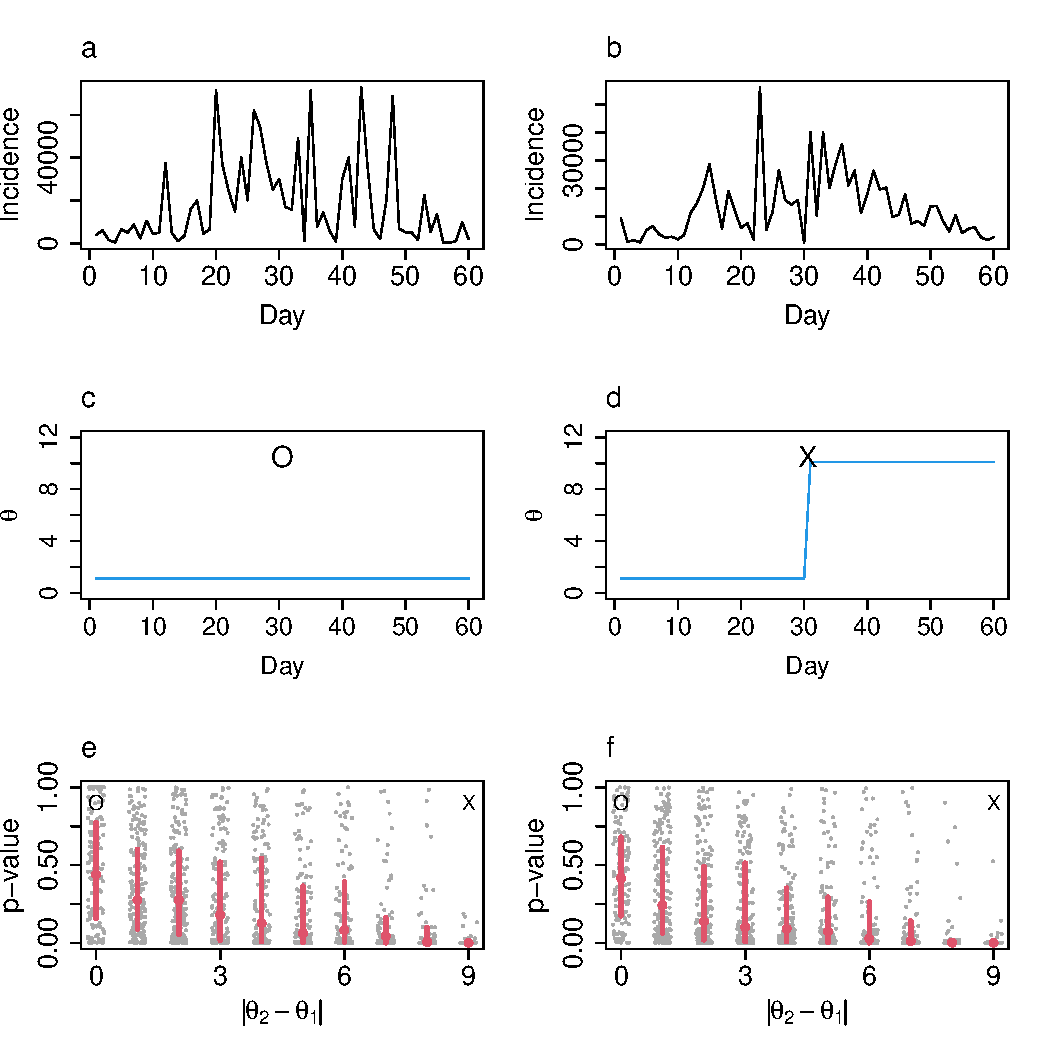
\includegraphics[width=1\textwidth]{fig1}
\caption{
Detecting dispersion changes in incidence time series in populations of different sizes. a: Simulated incidence when dispersion is constant. b: Simulated incidence when dispersion changes. c: Constant dispersion parameter used in generation of the above. d: Changing dispersion parameter used in generation of the above. e, f: Performance of the LRT with simulated data that have different absolute differences in \begin{math}\theta\end{math} (horizontal axis of each panel) illustrates p-value distribution in population size of 50,000 (e) and population size of 10,000,000 (f), which represent the range in the empirical data. O and X mark the null and alternative hypotheses indicated in panels c and d. Red vertical lines represent the interquartile range. 
 }
\label{fig1}
\end{figure}

The negative binomial framework for estimating \begin{math}\theta\end{math} is robust across the population sizes examined, and a large portion of inaccurate estimates correspond to small counties outside of the range considered (\nameref{S1_Fig}).
In row one and two of Fig.\ 1, we illustrate that an increase in \begin{math}\theta\end{math} is associated with decreased variability in simulated incidence time series. This pattern is observed in the empirical data, and is independent of whether incidence increases or decreases, as seen in Fig.\ 2.

\begin{figure}[!h]
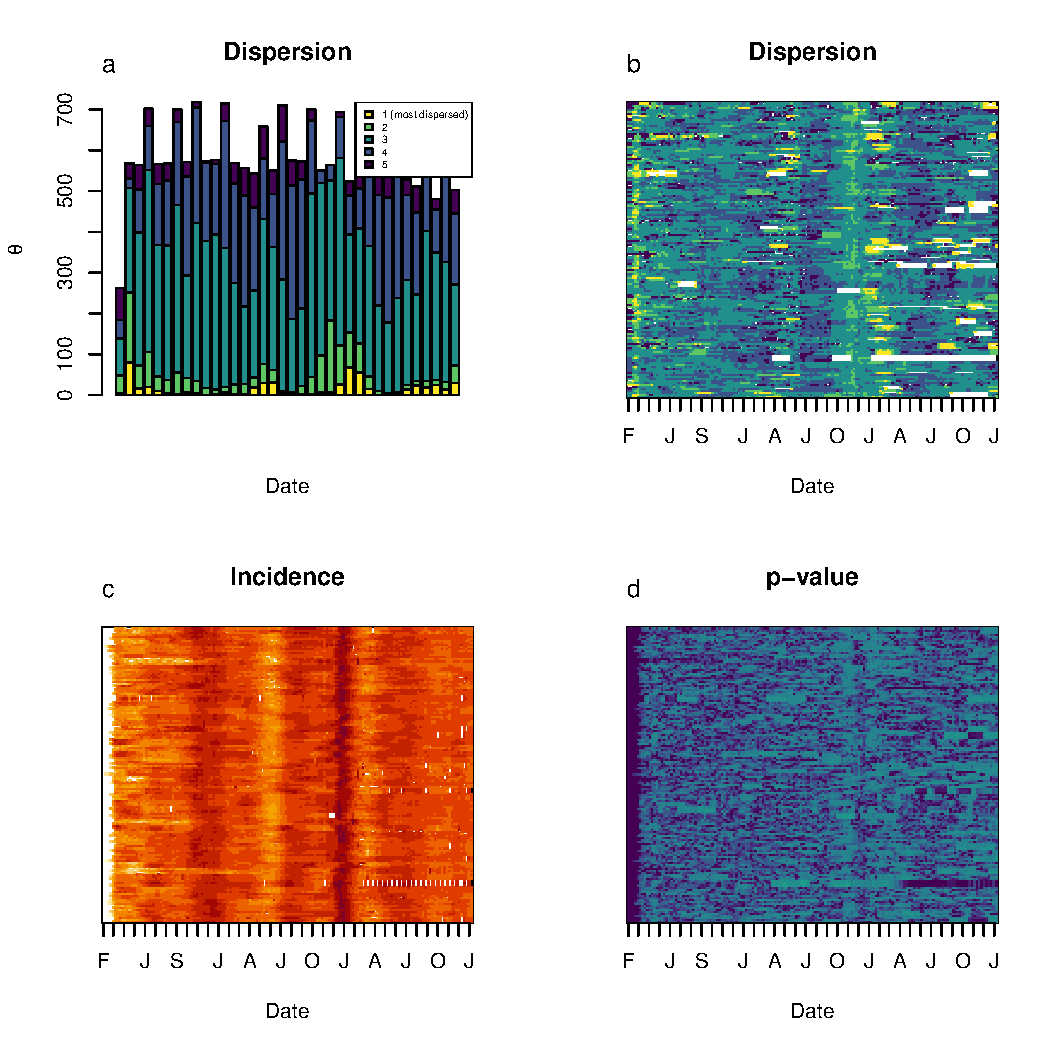
\includegraphics[width=1\textwidth]{fig2.pdf}
\caption{Negative binomial regression/LRT method applied to case counts between 2020-01-04 and 2023-03-18 from Jefferson County, AL. a: Case counts. b: Time series of $log_{10}\theta$ colored by whether the associated LRT statistic is greater than the Bonferroni-corrected level 0.05 quantile of a chi-square random variable with one degree of freedom (red indicates areas of putative change in $\theta$). The black line indicates the dispersion parameter under the model from Equation 1.
}
\label{fig2}
\end{figure}

Highly overdispersed incidence patterns were observed for many counties more frequently later in time series, consistent with more heterogeneity in transmission, susceptibility and reporting. 
The most dispersed category in Fig.\ 3 (e) reaches its highest proportion near the end of the time frame examined.
In addition, there are increases in dispersion around the peaks in incidence in the dataset (Fig. 3 c, d).
The evidence for a change in \begin{math}\theta\end{math} was observed across many counties (evidenced by a concentration of low p-values around peak incidence) (Fig. 3 f).

\begin{figure}[!h]
\centering
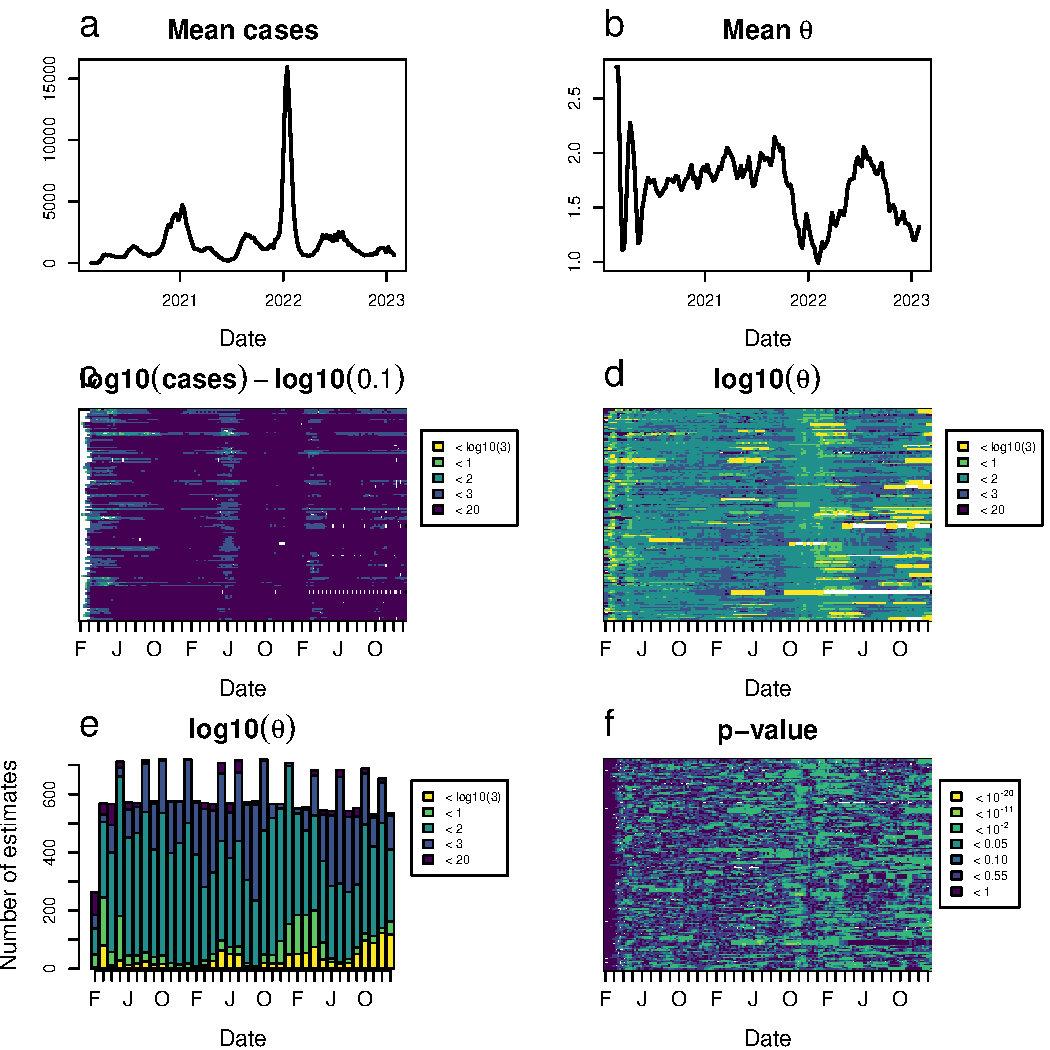
\includegraphics[width=0.85\textwidth]{fig3.pdf}
\caption{
Incidence and dispersion between 2020-01-04 and 2023-03-18 in large counties in the US. a: Mean COVID-19 cases of the 144 US counties over time. b: Mean $\theta$ of the 144 US counties over time. c: Case counts over time for each of the large counties (y-axis). d: $log_{10}\theta$ over time for each of the large counties (y-axis). e: Binned $log_{10}\theta$ over time. f: LRT p-values over time for each of the large counties (y-axis).
}
\label{fig3}
\end{figure}

Raising variance relative to mean (higher dispersion) implies spatiotemporal "crowding" of cases (i.e. localized surges) which may necessitate more surge capacity in hospitals and testing centers. Therefore, it may be the case that there were more surges on the way up to or on the way down from peak incidence. 
Additionally, it may indicate less diffuse epidemics that are potentially more subject to climate forcing \cite{dalziel_urbanization_2018}, or increased locally experienced mean density \cite{lloyd_mean_1967}. 

\section*{Discussion}
We presented an approach to quantify clustering of cases in epidemic time series that does not detect artifacts based on population size and incidence. 
Our method forms part of a larger push to investigate variability in incidence time series as an important attribute of epidemic time series using novel metrics.
For instance, burst-tree decomposition of time series’ has also facilitated computation of a burst-size distribution for a series given a specified time window \cite{jo_burst-tree_2020}, allowing comparison of variability within one location over time. 
Spatial variation in superspreading potential has been investigated through e.g., risk maps of superspreading environments \cite{loo_identification_2021}, so future work could investigate the correspondence between our variability metric and indicators of high risk of superspreading.
Methods that use incidence time series are crucial part due to the ease of obtaining incidence data, so the timing/geographical allocation of public health resources can be achieved with limited resources. 
Additionally, population-wide disease control approaches are often less effective than those which are targeted to individuals in high-transmission contexts \cite{lloyd-smith_superspreading_2005}, so models that incorporate transmission heterogeneity may catalyze the development of more efficient control strategies.
Our results imply that we can revise our understanding of case count dispersion: dispersion/crowding is high near peak incidence, suggesting that low dispersion is not simply governed by high incidence. 
Though large cities may be subject to more "smooth" epidemic dynamics, our contribution highlights the circumstances under which dynamics are less smooth in large counties. 
Previous research to evaluate bursty dynamics based on Influenza-like Illness (ILI) times series showed that epidemics in smaller communities are concentrated on narrower windows of the influenza season - the proportion of disease incidence that occurred in a given week was a metric of interest \cite{dalziel_urbanization_2018}. 
So, additional research is needed to understand the correspondence between burstiness of small communities and the potential impact of temporally changing dispersion in these areas.
%Though some kinds of time dependence in the rate can cause autocorrelation, as can contagion (if it occurs outside of set periods), and heterogeneity (if an omitted variable is correlated in time) \cite{barron_analysis_1992}, our focus on dispersion makes sense because we are concerned with the clustering of cases from the point of view of an individual case, which is caused by these factors operating within a set period. %Also, demographic structure (e.g., age structure) has the potential to affect temporal autocorrelation in transmission rate - the effects of age structure can be captured by a model that includes an infection rate that varies over time \cite{earn_dynamic_nodate}. 

\section*{Conclusion}
We presented an approach to quantify clustering of cases in epidemic time series that does not detect artifacts based on population size and incidence. 
While our estimation framework facilitates comparision of dispersion between counties and also over time in a given county, our LRT framework additionally allows for detection of changing dispersion. 
Application of these methods to empirical case count time series spanning from the beginning of 2020 to early 2023 revealed distinct increases in dispersion both near the end of the time window and near peaks in COVID-19 incidence. 
These findings will assist in the allocation of public health resources, especially in the planning of surge capacity. Since there are regimes of the COVID-19 epidemic that are subject to increased dispersion across large counties, these may be candidate time periods for rolling out extra capacity. However, further research is needed to understand this phenomemon in small counties, as well as for other pathogens.

\section*{Supporting information}

% Include only the SI item label in the paragraph heading. Use the \nameref{label} command to cite SI items in the text.
\paragraph*{S1 Fig.}
\label{S1_Fig}
{\bf Estimates of the dispersion parameter from simulated data.} Points colored red for underlying population sizes less than 50,000.
\begin{figure}[!h]
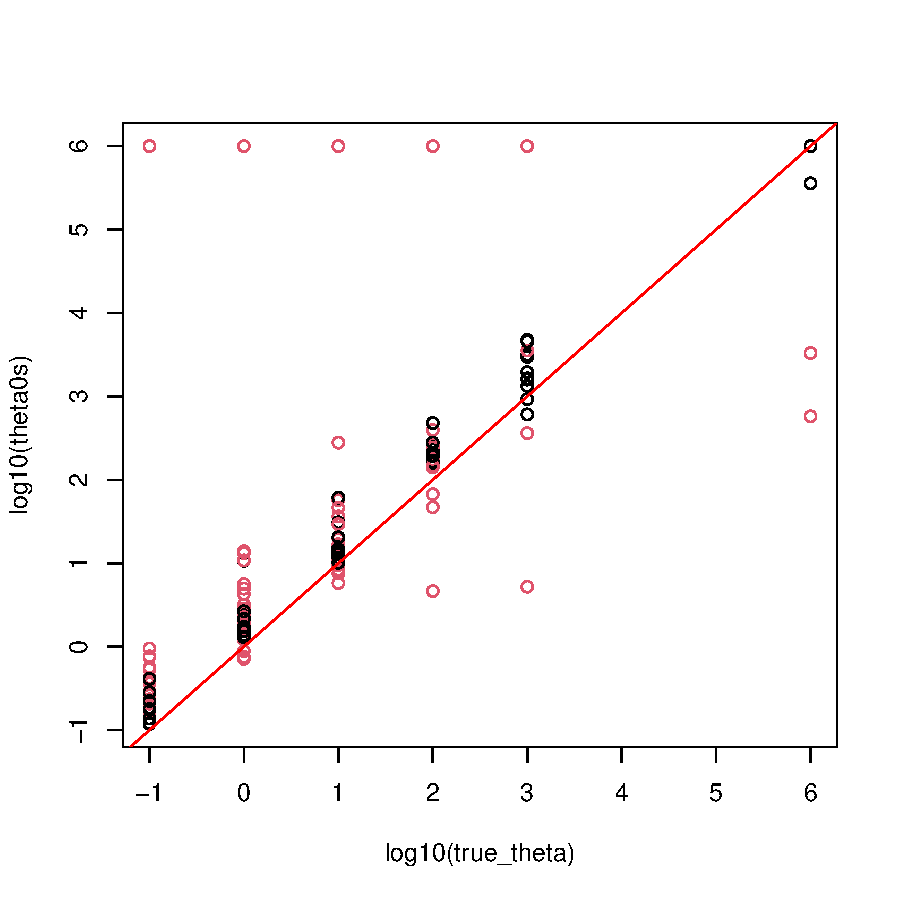
\includegraphics[width=0.6\textwidth]{thetaest_v_theta.pdf}
\label{S1}
\end{figure}

%\paragraph*{S2 Fig.}
%\label{S2_Fig}
%{\bf Lorem ipsum.} Analytical approach: robust to population size changes.

%\paragraph*{S1 File.}
%\label{S1_File}
%{\bf Lorem ipsum.}  Maecenas convallis mauris sit amet sem ultrices gravida. Etiam eget sapien nibh. Sed ac ipsum eget enim egestas ullamcorper nec euismod %ligula. Curabitur fringilla pulvinar lectus consectetur pellentesque.

%\paragraph*{S1 Video.}
%\label{S1_Video}
%{\bf Lorem ipsum.}  Maecenas convallis mauris sit amet sem ultrices gravida. Etiam eget sapien nibh. Sed ac ipsum eget enim egestas ullamcorper nec euismod %ligula. Curabitur fringilla pulvinar lectus consectetur pellentesque.

%\paragraph*{S1 Appendix.}
%\label{S1_Appendix}
%{\bf Lorem ipsum.} Maecenas convallis mauris sit amet sem ultrices gravida. Etiam eget sapien nibh. Sed ac ipsum eget enim egestas ullamcorper nec euismod %ligula. Curabitur fringilla pulvinar lectus consectetur pellentesque.

%\paragraph*{S1 Table.}
%\label{S1_Table}
%{\bf Lorem ipsum.} Maecenas convallis mauris sit amet sem ultrices gravida. Etiam eget sapien nibh. Sed ac ipsum eget enim egestas ullamcorper nec euismod %ligula. Curabitur fringilla pulvinar lectus consectetur pellentesque.

\section*{Acknowledgments}

\nolinenumbers

% Either type in your references using
% \begin{thebibliography}{}
% \bibitem{}
% Text
% \end{thebibliography}
%
% or
%
% Compile your BiBTeX database using our plos2015.bst
% style file and paste the contents of your .bbl file
% here. See http://journals.plos.org/plosone/s/latex for 
% step-by-step instructions.
% 
\bibliography{references}



\end{document}